\documentclass{beamer}

\usepackage{xeCJK}
\usepackage{amsmath, amssymb, blkarray, bm, cases, mathtools, nicefrac}
\usepackage[Symbol]{upgreek}
\usepackage[font=small]{caption}
\usepackage{XCharter, fouriernc}

\renewcommand{\today}{\number\year 年 \number\month 月}
\renewcommand{\figurename}{图}
\renewcommand{\tablename}{表}

\setCJKmainfont[BoldFont=WenQuanYi Micro Hei]{WenQuanYi Micro Hei Light}

\usetheme{default}
\usecolortheme{default}

\title{面向视觉惯性SLAM的通用\\增量式集束调整框架}
\author{王儒}
\institute{浙江大学CAD\&CG国家重点实验室}
\date{\today}

\begin{document}

\frame{\titlepage}

\begin{frame}
    \frametitle{大纲}
    \begin{enumerate}
        \item 研究背景
        \item 研究方法和内容
            \begin{itemize}
                \item 框架
                \item HLMDL
                \item PBT回代算法
            \end{itemize}
        \item 实验结果和分析
        \item 展望和致谢
    \end{enumerate}
\end{frame}

\begin{frame}
    \frametitle{研究背景}
    \framesubtitle{SLAM系统中的状态估计问题}
    \begin{enumerate}
        \item 非线性高斯系统的最大后验估计
        \item 问题形式(因子图)
        \item 状态估计的求解要求:实时、合理精度范围
    \end{enumerate}
\end{frame}

\begin{frame}
    \frametitle{研究背景}
    \framesubtitle{传统批量式集束调整方法}
    \begin{enumerate}
        \item BA:最小二乘和图优化
        \item 相关工作:Ceres-Solver,G2O
    \end{enumerate}
\end{frame}

\begin{frame}
    \frametitle{研究背景}
    \framesubtitle{现有BA求解器的缺点}

    减小BA问题规模:
    \begin{enumerate}
        \item 批量BA时间复杂度:$O(N^3)$,大量重复计算
        \item G2O接口奇怪,代码恶心,没有文档,速度稍快
        \item 可定制性低
    \end{enumerate}
\end{frame}

\begin{frame}
    \frametitle{研究背景}
    \framesubtitle{SLAM中BA加速思路}

    在不改变BA问题的前提下加快求解
    \begin{itemize}
        \item 利用稀疏性
        \item 保持稀疏性:变量排序(COLAMD、CHOLMOD)、分组(舒尔补)
        \item 减少重复计算:增量式BA
    \end{itemize}
\end{frame}

\begin{frame}
    \frametitle{研究方法和内容}
    \framesubtitle{面向视觉惯性SLAM的通用增量式集束调整框架}
    \begin{figure}[h]
        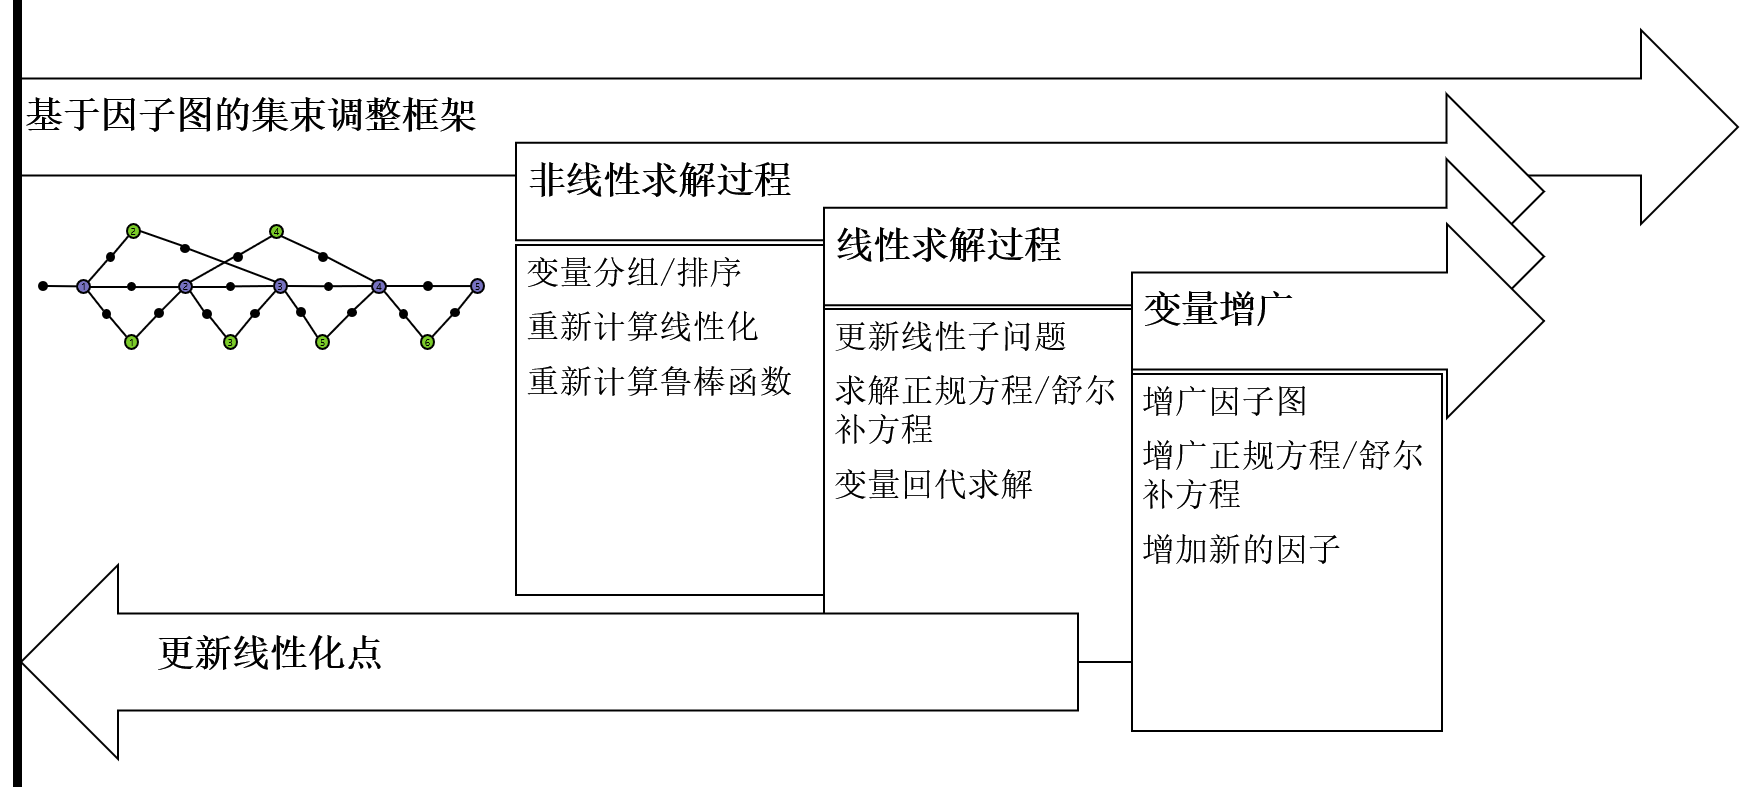
\includegraphics[width=.8\textwidth]{figs/framework.png}
        \caption{增量式BA基本求解流程}
        \label{fig:framework}
    \end{figure}
\end{frame}

\begin{frame}
    \frametitle{研究方法和内容}
    \framesubtitle{通用增量式BA框架架构}
    \begin{enumerate}
        \item 非线性部分:基于因子图的增量舒尔补;内置常用factor并支持自定义
        \item 线性求解:HLMDL算法;内置I-PCG算法和Cholesky算法并允许自定义
        \item 线性回代:基于PBT的变量回代方法
    \end{enumerate}
\end{frame}

\begin{frame}
    \frametitle{研究方法和内容}
    \framesubtitle{通用增量式BA框架架构}

    非线性部分
    \begin{itemize}
        \item 基于因子图的增量舒尔补
        \item 内置常用factor并支持自定义
    \end{itemize}
\end{frame}

\begin{frame}
    \frametitle{研究方法和内容}
    \framesubtitle{通用增量式BA框架架构}

    线性部分
    \begin{itemize}
        \item 回顾LM和DL
        \item 针对DL中rank-deficient问题提出HLMDL
        \item 给出条件数对比
    \end{itemize}
\end{frame}

\begin{frame}
    \frametitle{研究方法和内容}
    \framesubtitle{通用增量式BA框架架构}

    线性回代部分
    \begin{itemize}
        \item 增量舒尔补效果不好——分析可得发现变量不一致问题
        \item 提出基于PBT的回代算法,分析对比PBT形状
        \item 给出对比
    \end{itemize}
\end{frame}

\begin{frame}
    \frametitle{实验结果和分析}
    结果+分析
\end{frame}

\begin{frame}
    \frametitle{未来工作展望}
    \begin{enumerate}
        \item 回路闭合
        \item 状态边缘化会影响稀疏性
        \item 进一步增量化
        \item 并行算法
    \end{enumerate}
\end{frame}
